%\documentclass[cjk,slidestop,compress,mathserif,blue]{beamer}
\documentclass[cjk,slidestop,handout,compress,mathserif,blue]{beamer}	%打印PPT用,handout(讲义)可去掉过渡效果,如\pause引起的多页显示,为打印时节省纸张
%dvipdfm选项是关键,否则编译统统通不过
%beamer的颜色选项定义的是导航条和标题的颜色(即关键词structure的颜色)

%%%%%%%%%%%%%%%%仅限于XeTeX可使用的宏包%%%%%%%%%%%%%%%%%%%%%%%%%%%%
\usepackage{fontspec,xunicode,xltxtra,beamerthemesplit}
%\usepackage{beamerthemesplit}
\usepackage{xeCJK}
\setCJKmainfont[BoldFont=黑体, ItalicFont=楷体, BoldItalicFont=仿宋]{黑体}
%\setsansfont[Mapping=tex-text]{Adobe 黑体 Std}
%如果装了Adobe Acrobat,可在font.conf中配置Adobe字体的路径以使用其中文字体
%也可直接使用系统中的中文字体如SimSun,SimHei,微软雅黑 等
%原来beamer用的字体是sans family;注意Mapping的大小写,不能写错

%%%%%%%%   确定标题和导航条结构的框架     %%%%%%%%%%%%
\usepackage{beamerthemeshadow}                       %
%\usepackage{beamerthemeclassic}%导航条色与背景色一致%
%%%%%%%%%%%%%%%%%%%%%%%%%%%%%%%%%%%%%%%%%%%%%%%%%%%%%%
\setbeamerfont{roman title}{size={}}
%\usepackage{CJK} % CJK 中文支持                                  %
\usepackage{amsmath,amsthm,amsfonts,amssymb,bm}
\usepackage{mathrsfs}
\usepackage{xcolor}                                        %使用默认允许使用颜色
\usepackage{hyperref} 
\usepackage{graphicx}
\usepackage{subfigure}           %图片跨页

%\usepackage[numbers,sort&compress]{natbib} %紧密排列             %
\usepackage[sectionbib]{chapterbib}        %每章节单独参考文献   %
\usepackage{hypernat}                                                                         %
%\usepackage[dvipdfm,bookmarksopen=true,pdfstartview=FitH,CJKbookmarks]{hyperref}		%
\hypersetup{bookmarksnumbered,colorlinks,linkcolor=brown,citecolor=blue,urlcolor=red}         %
%参考文献含有超链接引用时需要下列宏包,注意与natbib有冲突        %
%\usepackage[dvipdfm]{hyperref}                                  %
%\usepackage{hypernat}                                           %
\newcommand{\upcite}[1]{\hspace{0ex}\textsuperscript{\cite{#1}}} %

%\useoutertheme{smoothbars}
\useinnertheme[shadow=true]{rounded}
\usetheme{Berkeley}                                          %主题式样
%\usetheme{Luebeck}

\usecolortheme{lily}                                        %颜色主题式样

\usefonttheme{professionalfonts}                           %字体主题样式宏包

%\beamertemplatetransparentcoveredhigh                      %使所有被隐藏的文本高度透明
\beamertemplatetransparentcovereddynamicmedium             %使所有被隐藏的文本完全透明,动态,动态的范围很小
\mode<presentation>
%\beamersetaveragebackground{gray}                          %设置背景颜色(单一色) 
\beamertemplateshadingbackground{green!10}{red!5}         %设置背景颜色(渐变色)

%在指定位置精确放置logo
\usepackage{tikz}
\usepackage{beamerfoils}
\usepackage{pgf}
\logo{\pgfputat{\pgfxy(11.68,0.15)}{
\includegraphics[height=1.01cm,viewport=0 0 140 120,clip]{Figures/BCC_logo-1.png}}\pgfputat{\pgfxy(10.502,-0.218)}{
\includegraphics[height=0.369cm,viewport=140 0 540 120,clip]{Figures/BCC_logo-1.png}}}
%\logo{\pgfputat{\pgfxy(11.68,0.15)}{
\includegraphics[height=0.95cm,viewport=0 0 510 360,clip]{Figures/Logo_Gainstrong.png}}\pgfputat{\pgfxy(10.333,-0.195)}{
\includegraphics[height=0.35cm,viewport=530 70 1100 218,clip]{Figures/Logo_Gainstrong.png}}}
%\MyLogo{
%	\pgfputat{\pgfxy(-50,-50)}{\pgfbox[right,base]{
\includegraphics[height=1cm]{Figures/BCC_logo-1.png}}}
%logo作为背景放置
%\setbeamertemplate{background}{
%	\pgfputat{\pgfxy(6.5,-0.5)}{\pgfbox[left,top]{\pgfimage[height=1.1cm]{Figures/BCC_logo-1.png}}}}

%\logo{}									%不显示logo

\begin{document}
%\begin{CJK*}{GBK}{song}
%\begin{CJK*}{GBK}{kai}
%beamer下不能用\songyi、\zihao等命令!
%\graphicspath{Figures/}

%-------------------------------PPT Title-------------------------------------
\title{课题一}
%-----------------------------------------------------------------------------

%----------------------------Author & Date------------------------------------
\author{北京市计算中心\:\:姜骏}
%\date{\textrm{清华大学\:\:物理系\vskip 5pt 2017.01.20-22}}
\date{2017.03.02}
\frame{\titlepage}
%-----------------------------------------------------------------------------

%------------------------------------------------------------------------------列出全文 outline ---------------------------------------------------------------------------------
\section*{}
\frame[allowframebreaks]
{
  \frametitle{Outline}
%  \frametitle{\textcolor{mycolor}{\secname}}
  \tableofcontents%[current,currentsection,currentsubsection]
}
%在每个section之前列出全部Outline
%类似的在每个subsection之前列出全部Outline是\AtBeginSubsection[]
\AtBeginSection[]
{
  \frame<handout:0>
  {
    \frametitle{Outline}
%全部Outline中,本部分加亮
    \tableofcontents[current,currentsection]
  }
}

%------------------------------------------------------------------------------PPT main Body------------------------------------------------------------------------------------
\small
\section{主体框架与软件}
\frame
{
	\frametitle{计算主体框架的基本构想}
	\begin{itemize}
		\item 统一的高通量自动流程的数据格式
		\item 自动执行的多尺度、高通量计算流程,实现多组元材料体系从微观到宏观的结构、物性和服役行为的全链条多尺度集成计算
		\item 多尺度、高通量、高并发计算过程中不同计算任务间的高效信息传递、储存
		\item 规范定义不同模块间的I/O接口,搭建集成计算环境框架
	\end{itemize}
\begin{figure}[h!]
\centering
\vspace*{-0.2in}
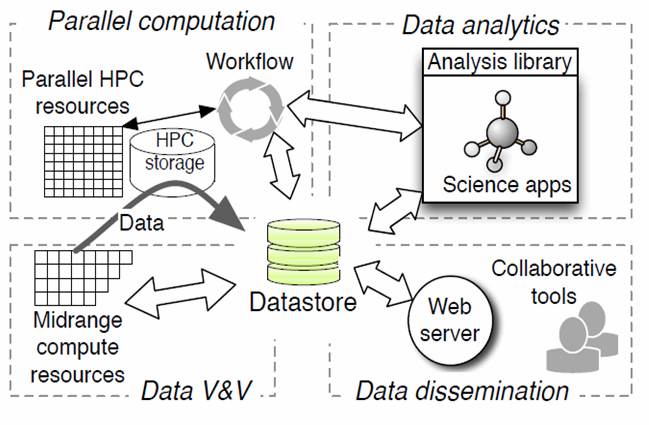
\includegraphics[height=1.3in,width=2.0in,viewport=0 0 680 460,clip]{Figures/Parallel_computation.png}
\caption{\fontsize{5.2pt}{2.5pt}\selectfont{\textrm{High throughput architecture. The datastore serves all four functions, clockwise from upper-left:~Parallel computation, Data analytics, Data dissemination, and Data validation and verification. Ref\cite{unpublished}}}}%
\label{parallel_computation}
\end{figure} 
}

\frame
{
	\frametitle{国内外已有的计算平台}
\begin{figure}[h!]
\centering
\vspace{-15.5pt}
\subfigure[\fontsize{7.5pt}{6.2pt}\selectfont{\textrm{Auto-FLOW (AFLOW)}\upcite{CMS58-227_2012}}]{
\label{AFLOW_data_flow}
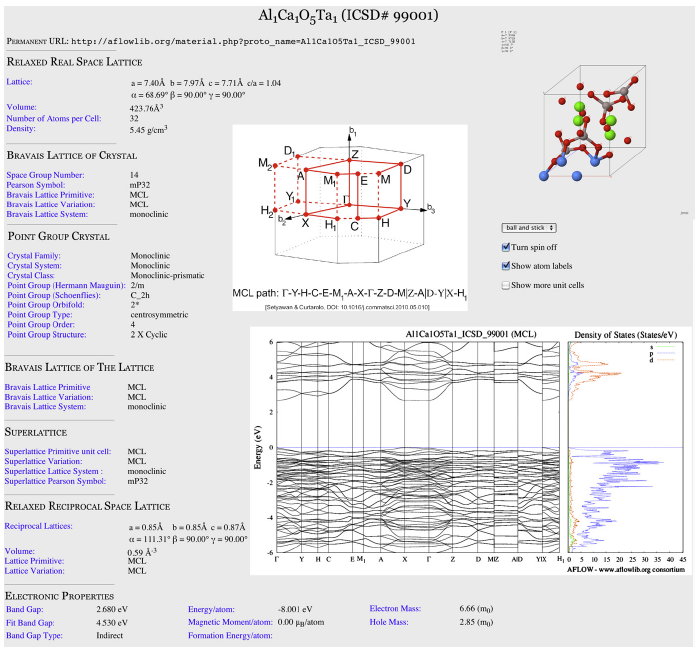
\includegraphics[height=1.2in,width=1.6in,viewport=0 0 720 660,clip]{Figures/AFLOW_database.png}}
\subfigure[\fontsize{7.5pt}{6.2pt}\selectfont{\textrm{Material Project (MP)}\upcite{CMS97-209_2015}}]{
\label{MP_commp_infrastructure}
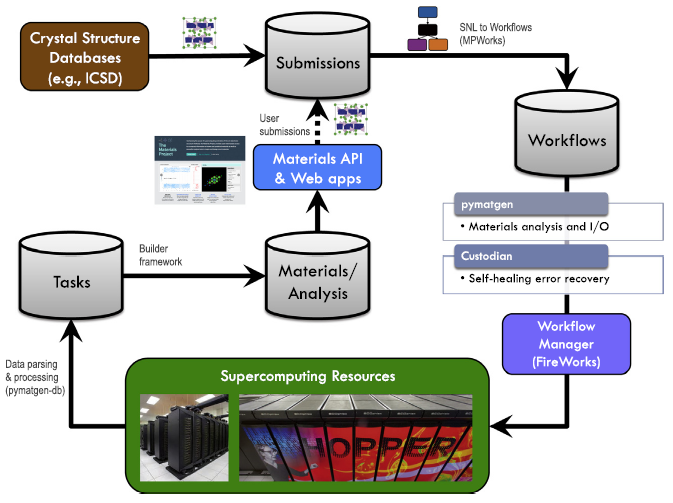
\includegraphics[height=1.2in,width=1.7in,viewport=0 0 670 530,clip]{Figures/MP_comp_infrastructure.png}}
\subfigure[\fontsize{3.5pt}{3.2pt}\selectfont{\textrm{Quantum Materials Informatics Project (QMIP)}\upcite{url_QMIP}}]{
\label{QMIP_Shame}
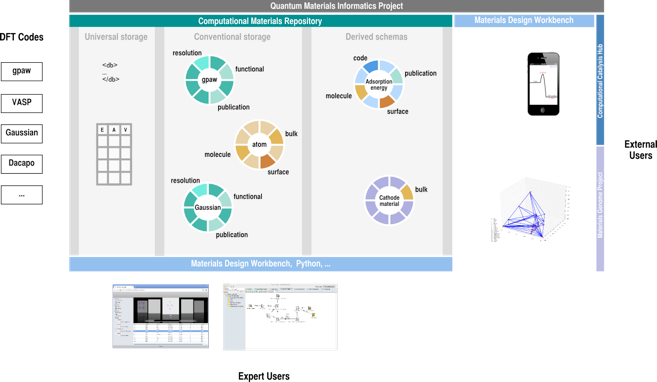
\includegraphics[height=1.2in,width=1.7in,viewport=0 0 670 420,clip]{Figures/QMIP_shame.png}}
\subfigure[\fontsize{6.5pt}{5.2pt}\selectfont{\textrm{Clean Energy Project (CEP)}\upcite{JPCL2-2241_2011}}]{
\label{CEP_structure_flow}
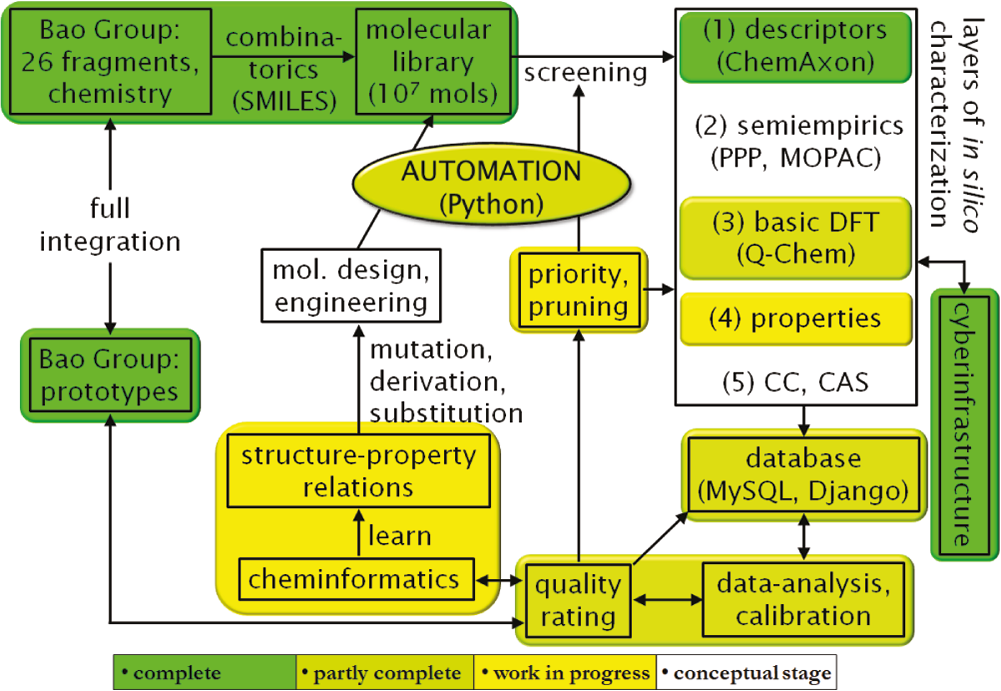
\includegraphics[height=1.2in,width=1.6in,viewport=0 0 1020 730,clip]{Figures/CEP_structure_flow.png}}
%\caption{}%
\label{Auto_Flow_Platform}
\end{figure}
}

\frame
{
	\frametitle{\textrm{计算平台}}
\begin{figure}[h!]
\centering
\vspace*{-0.2in}
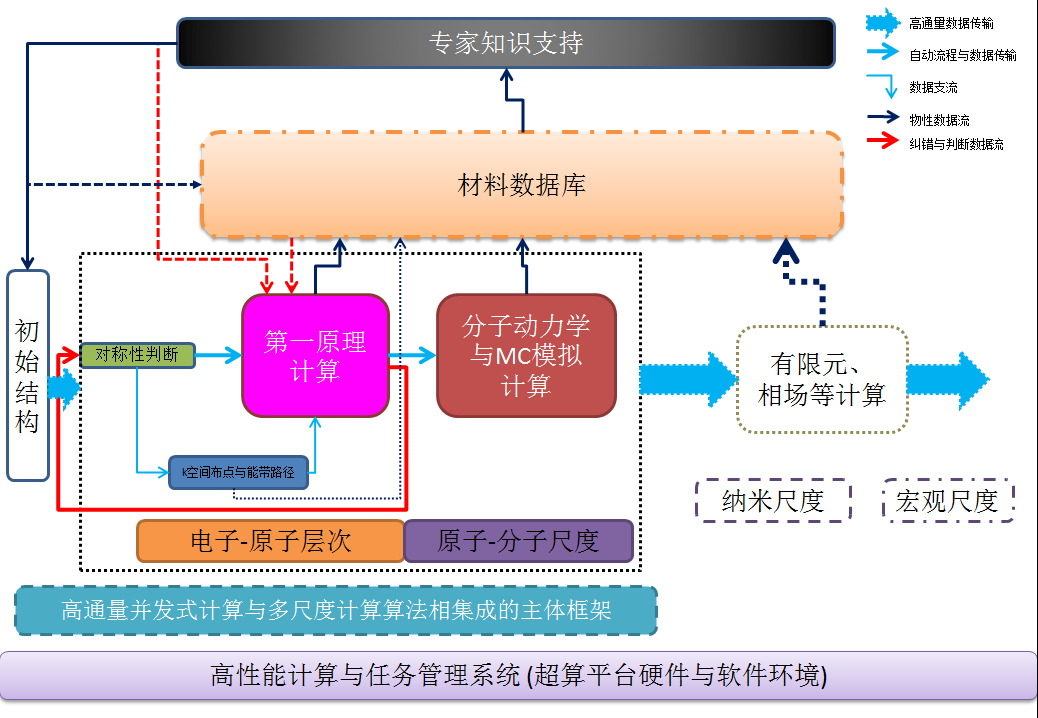
\includegraphics[height=2.6in,width=3.6in,viewport=0 0 1038 730,clip]{Figures/Auto_Flow.png}
\caption{\fontsize{7.2pt}{4.2pt}\selectfont{\textrm{The schematic framework and platform of our project.}}}%
\label{Auto_Flow}
\end{figure} 
}

\section{材料计算中的对称性问题}
\frame
{
	\frametitle{对称性模块的功能}
	对称性模块与电子结构计算
	\begin{itemize}
		\item \textcolor{blue}{第一原理计算中,材料的初始结构经过结构弛豫会导致晶胞参数和原子坐标发生改变,对称性也将发生变化。}
		\item \textcolor{blue}{材料的电子能带结构表示与体系的对称性密切关联}
	\end{itemize}
	\vskip 30pt
	高通量自动流程中的对称性模块
	\begin{itemize}
		\item \textcolor{blue}{高通量计算中,利用对称性可以在保证计算精度的同时,有效地降低计算量}
		\item \textcolor{blue}{没有完整的材料结构数据库支持,第一原理“结构弛豫-静态计算-能带表示”自动流程闭环必须有对称性模块支持}
	\end{itemize}
}

\frame
{
	\frametitle{传统能带计算的问题}
	对称性相同的材料电子结构表现出明显的相似性,但传统能带计算和表示的$\vec k$点路径($\vec k$-\textrm{Path})选择有着明显的人为性和任意性
%\vspace{10pt}
\begin{figure}[h!]
\centering
\hspace*{-0.30in}
\subfigure[\fontsize{6.5pt}{5.2pt}\selectfont{\textrm{Brillouin Zone of BCC lattice}}]{
\label{Brillouin_Zone_BCC}
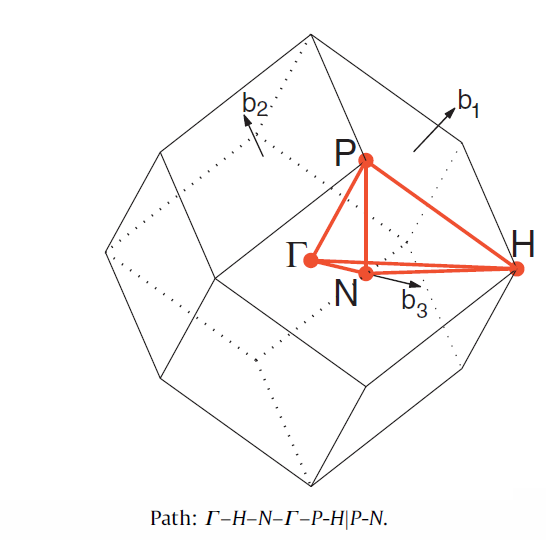
\includegraphics[height=1.5in,width=1.6in,viewport=00 0 550 520,clip]{Figures/Brillouin-Zone_BCC.png}}
%\vskip 0.10in
\subfigure[\textrm{Band structure of GeF$_4$}]{
\label{Band_Gap_GeF4}
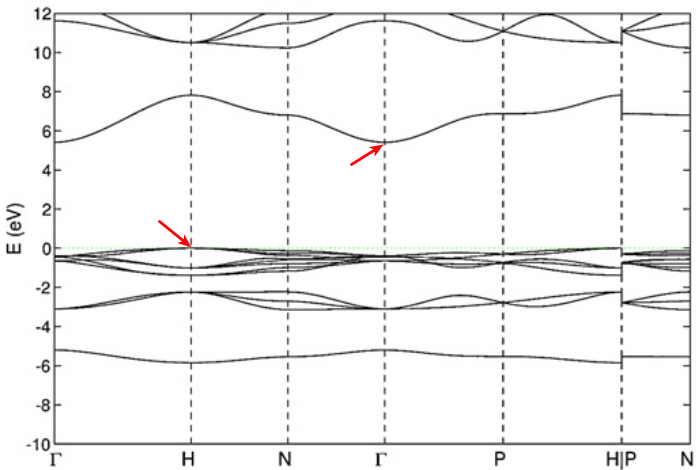
\includegraphics[height=1.05in,width=1.65in,viewport=0 0 750 500,clip]{Figures/Band-Struct_GeF4.png}}
\label{Band_Gap_BCC_GeF4}
\end{figure}
利用对称性模块实现\textcolor{red}{能带表示路径~$\vec k$-\textrm{path}“标准化”},对于高通量材料电子结构数据挖掘有着重要意义
}

\frame
{
	\frametitle{标准化的对称性模块}
\begin{enumerate}
   \setlength{\itemsep}{20pt}
	\item 结构文件转换子模块:~\textcolor{magenta}{不同格式的结构文件间的相互转换}
	\item 对称性分析功能子模块
		\begin{itemize}
			\item 确定原胞的点群、空间群和对称操作矩阵
			\item 标准化的初基原胞(\textrm{primitive cell})
				\vskip 2pt
				\textcolor{magenta}{按晶轴长度和晶面夹角的大小确定晶格矢量排列顺序}
		\end{itemize}
	\item 标准化$\vec k$~点生成子模块\upcite{CMS49-299_2010}
		\begin{itemize}
			\item 确定14种\textrm{Bravais~}格子所有标准化\textrm{Wigner-Seitz~}原胞
			\item 确定所有高对称性点的分数坐标和能带图中$\vec k$-\textrm{path}
		\end{itemize}
	\item 标准化结构参数的数据存储:~\textcolor{magenta}{元素、晶格、对称性等信息}
\end{enumerate}
}

\frame
{
	\frametitle{标准化结构参数的数据存储子模块}
\begin{figure}[h!]
\centering
\vspace*{-0.2in}
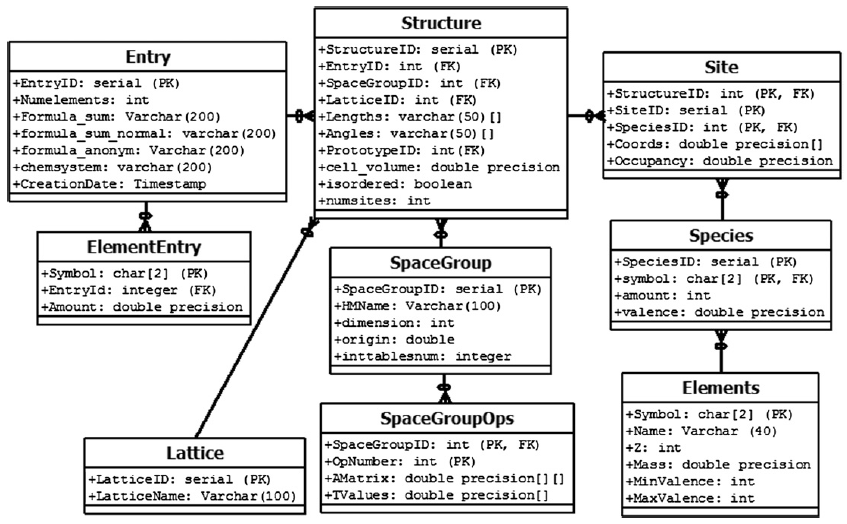
\includegraphics[height=2.5in,width=3.7in,viewport=0 0 850 540,clip]{Figures/MP_database_structure.png}
\caption{\fontsize{7.2pt}{4.2pt}\selectfont{\textrm{Basic database schema for storing periodic crystal structures. Ref\cite{CMS50-2295_2011}}}}%
\label{MP_structure_data}
\end{figure} 
}

\section{自动纠错与单线程加速}
%\frame
%{
%	\frametitle{自动流程\textrm{Fireworks}}
%\begin{figure}[h!]
%\centering
%\vspace*{-0.1in}
%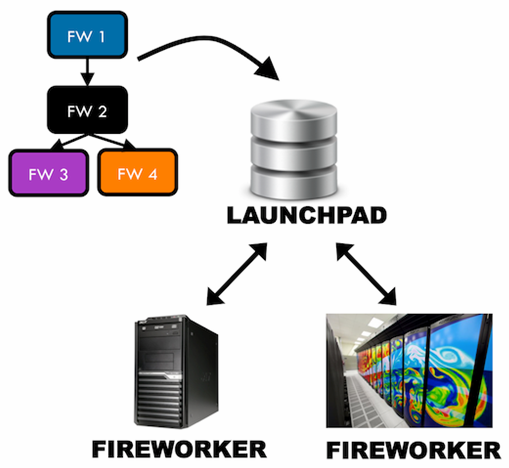
\includegraphics[height=2.5in,width=2.5in,viewport=0 0 500 500,clip]{Figures/MP_fireworks.png}
%\caption{\fontsize{7.2pt}{4.2pt}\selectfont{\textrm{Schematic representation of the Fireworks of Materials Project.}}}%
%\label{MP_firework}
%\end{figure} 
%}
%
\frame
{
	\frametitle{自动纠错}
		\begin{figure}[h!]
			\begin{minipage}[t]{0.50\linewidth}
		高通量计算错误的主要来源
\begin{itemize}
	\item \textcolor{violet}{硬件与系统软件层次}\\
		作业管理系统调度和维护
	\item \textcolor{violet}{核心软件层次}\\
		核心软件的错误输出与提示
	\item \textcolor{violet}{应用层次}\\
		核心软件计算参数设置不合理\textcolor{red}{(材料计算专家经验集成)}
\end{itemize}
		解决方案
		\begin{itemize}
			\item 作业进程错误断点守护
			\item 专家经验程序化,\textcolor{blue}{重点围绕核心计算参数的优化选择}
			\item 计算作业重启动
		\end{itemize}<++>
			\end{minipage}
			\hfill
			\begin{minipage}[t]{0.45\linewidth}
				\centering
				\vspace*{-0.3in}
				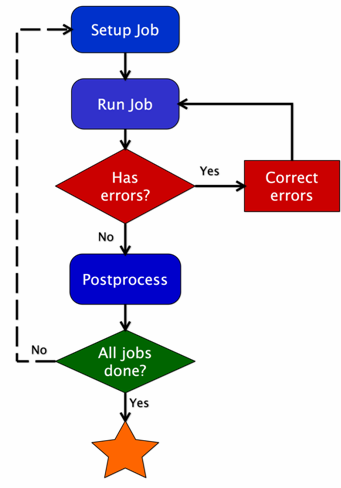
\includegraphics[height=2.4in,width=1.5in,viewport=0 0 350 520,clip]{Figures/MP_custodian.png}
				\caption{\fontsize{7.2pt}{4.2pt}\selectfont{\textrm{Schematic representation of the Custodian of Materials Project.}}}%
				\label{MP_custodian}
			\end{minipage}
				%\hspace*{-10pt}
		\end{figure} 
}

\frame
{
	\frametitle{单线程加速建议}
	第一原理计算核心程序的迭代与弛豫是计算中的主要耗时部分,优化和改进这部分核心程序单线程速度,建议主要从以下角度考虑
	\begin{itemize}
   		\setlength{\itemsep}{20pt}
		\item 第一原理核心程序计算过程中使用大量的\textrm{FFT~}变换,优化和提升\textrm{FFT~}变换效率
		\item 核心计算程序(包括第一原理和分子动力学)考虑\textrm{GPU~}计算对加速
	\end{itemize}
}
%\frame
%{
%\frametitle{发展统一理论框架下的材料计算程序}
%\begin{itemize}
%	\item
%\end{itemize}
%}

%\appendix
%------------------------------------------------------------------------Reference----------------------------------------------------------------------------------------------
%\begin{thebibliography}{99}
%-----------------------------------------------------------------------------------------------------------------------------------------------------------------------%
%\frame
%{
%\frametitle{主要参考文献}
%{\small
%\bibitem{Singh_Book}\textrm{D. J. Singh. \textit{Plane Wave, PseudoPotential and the LAPW method} (Kluwer Academic, Boston,USA, 1994)}					%
%  \nocite{*}																				%
%}
%}
%\end{thebibliography}
\begin{thebibliography}{99}
\frame
{
\frametitle{主要参考文献}
\fontsize{7.5pt}{3.9pt}\selectfont{
%	\bibitem{Huang_Han}黄昆\:原著、韩汝琦\:改编, {\textit{固体物理学}}\:高等教育出版社, 北京, 1988
%	\bibitem{Xie_Lu}谢希德、陆栋\:主编, {\textit{固体能带理论}}\:复旦大学出版社, 上海, 1998
%	\bibitem{url_Mater_Genome}\textrm{\url{https://www.whitehouse.gov/sites/default/files/microsites/ostp/materials_genome_initiative-final.pdf}}
	\bibitem{unpublished}\textrm{D. Gunter, S. Cholia, A. Jain, M. Kocher, K. Persson, L. Ramakrishnan, S. P. Ong and G. Ceder. \textit{Community Accessible Datastore of High-Throughput Calculations: Experiences from the Materials Project} (unpublished)}
	\bibitem{CMS58-227_2012}\textrm{S. Curtarolo, W. Setyawan, S. Wang, J. Xue, K. Yang, R. H. Taylor, L. J. Nelson, G. L. Hart, S. Sanvito, M. Buongiorno-Nardelli, N. Mingo and O. Levy \textit{Comp. Mater. Sci.}, \textbf{58} (2012), 227}
	\bibitem{CMS97-209_2015}\textrm{S. P. Ong, S. Cholia, A. Jain, M. Brafman, D. Gunter, G. Ceder and K. A. Persson. \textit{Comp. Mater. Sci.}, \textbf{97} (2015), 209}
	\bibitem{url_QMIP}\textrm{\url{http://www.qmip.org/qmip.org/Welcome.html}}
	\bibitem{JPCL2-2241_2011}\textrm{J. Hachmann, R. Olivares-Amaya, S. Atahan-Evrenk, C. Amador-Bedolla, R. S. S$\acute{a}$nchez-Carrera, A. Gold-Parker, L. Vogt, A. M. Brockway and A. Aspuru-Guzik \textit{J. Phys. Chem. Lett.}, \textbf{2} (2011), 2241}
	\bibitem{CMS49-299_2010}\textrm{W. Setyawan and S. Curtarolo \textit{Comp. Mater. Sci.}, \textbf{49} (2010), 299}
	\bibitem{CMS50-2295_2011}\textrm{A. Jain, G. Hautier, C. J. Moore, S. P. Ong, C. C. Fischer, T. M. Kristin, K. A. Persson and G. Ceder \textit{Comp. Mater. Sci.}, \textbf{50} (2011), 2295}
}
\nocite*{}
}
\end{thebibliography}
%{\small
%\phantomsection\addcontentsline{toc}{section}{Bibliography}	 %直接调用\addcontentsline命令可能导致超链指向不准确,一般需要在之前调用一次\phantomsection命令加以修正	%
%\bibliography{Myref}																			%
%\bibliographystyle{mybib}																		%
%  \nocite{*}																				%
%}
%-----------------------------------------------------------------------------------------------------------------------------------------------------------------------%


%-----------------------------------------------------------Beamer下不建议使用bib,因为涉及分页--------------------------------------------------------------------------%
%{\small
%\phantomsection\addcontentsline{toc}{section}{Bibliography}	 %直接调用\addcontentsline命令可能导致超链指向不准确,一般需要在之前调用一次\phantomsection命令加以修正	%
%\bibliography{Myref}																			%
%\bibliographystyle{mybib}																		%
%  \nocite{*}																				%
%}

%------------------------------------------------------------------------------------------------------------------------------------------------------------------------------%

%-------------------------------------------------------------------------Thanks------------------------------------------------------------------------------------------------
%\section{致谢}
%\frame
%{
%\frametitle{致$\quad$谢}
%\begin{itemize}
%    \setlength{\itemsep}{20pt}
%  \item 感谢本团队高兴誉、吴泉生、宋红州等各位老师参与的讨论
%  \item 感谢莫所长、宋主任以及软件中心各位老师和同事
%  \item 感谢王崇愚先生的帮助
%\end{itemize}
%}

\logo{}									%不显示logo
%\frame
%{
%\vskip 60 pt
%%\hskip 10pt \textcolor{blue}{\Huge 感谢答辩委员会各位老师\,\textrm{!}}\\
%\vskip 35 pt
%\hskip 60pt \textcolor{blue}{\Huge 谢谢大家\:!}
%%\vskip 15 pt
%%\hskip 40pt \textcolor{blue}{\Huge \textrm{for your attention\:!}}
%}

%-------------------------------------------------------------------------------------------------------------------------------------------------------------------------------

\clearpage
%\end{CJK*}
\end{document}
